\section{Modello CMD e Destino dell'universo}\label{sec:modello-CDM-destino}

\subsection{Modello CMD}\label{sec:modello-CDM}
Riassumendo, il modello che è stato adottato oggi per descrivere il nostro universo prevede i seguenti punti chiave:
\begin{enumerate}
    \item la \textit{cold dark matter (materia oscura fredda, CMD)}è la componente principale della materia che compone l'universo;
    \item il nostro universo ha una geometria piatta generata da una fase inflazionaria primordiale;
    \item l'universo si sta espandendo con accelerazione costante, dipendente dalla costante cosmologica $\Lambda$, dovuta al dominio della componente di energia oscura sulle altre;
    \item le prime strutture cosmiche si sono formate come conseguenza dell' instabilità gravitazionale;
    \item la formazione delle galassie è una conseguenza dell'aggregazione barionica in buche di potenziale, dovute alla presenza di un alone di materia oscura.
\end{enumerate}

Questo modello descrive bene il nostro universo, ma non spiega la presenza di strutture come la materia o energia oscura, questo ci fa intendere che la relatività generale potrebbe non essere la teoria appropriata per studiare scale cosmologiche.

\subsection{Destino dell'universo}\label{sec:destino}

Dopo l'epoca della radiazione e della materia, sta cominciando la terza, e ultima, fase dell'evoluzione del nostro universo, in cui la componente dominante è quella dell'energia oscura. Il modello vuole che la densità di energia oscura sia stata costante durante tutta la vita dell'universo, ma che ora stia diventando dominante a causa della diminuzione di densità di materia e radiazione, come mostrato in figura~\ref{fig:epoche}, in un periodo relativamente recente ($z \sim 0.5$).

\begin{figure}
    \centering
    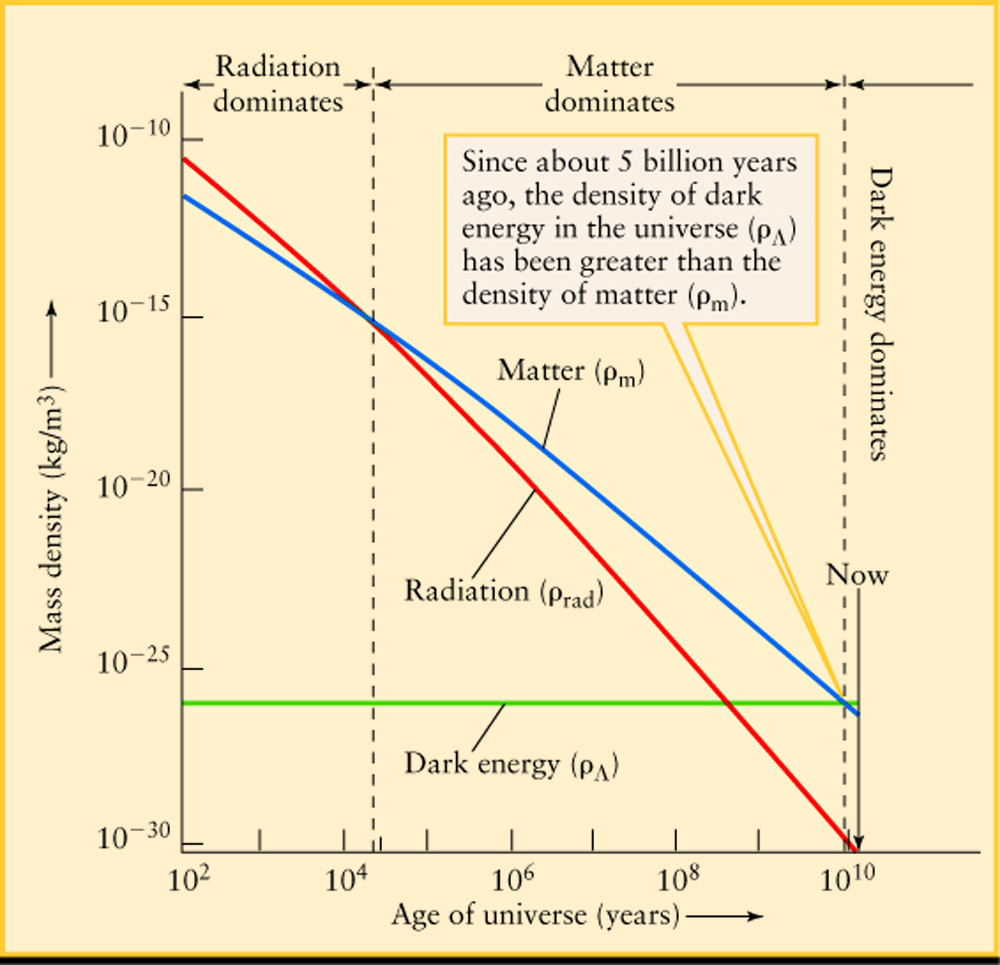
\includegraphics[width = 0.5\textwidth]{immagini/epoche-universo.png}
    \caption{La figura mostra l'andamento delle varie densità di massa di radiazione, materia ed energia oscura, rispettivamente rosso, blu e verde, assieme ai punti in cui cambia il dominio di una sull'altra.}\label{fig:epoche}
\end{figure}

A causa di ciò, l'universo è destinato ad espandersi con accelerazione sempre maggiore fino a raggiungere quella che viene chiamata morte dell'universo, a meno che l'ipotesi sulla relazione tra energia oscura e costante cosmologica non sia sbagliata.